%!TEX encoding = UTF-8 Unicode
\documentclass[12pt]{article} % 12pt-article hier, aber Abschlussarbeit dann 12pt-book
\usepackage[utf8]{inputenc}   %empfohlene Zeichenkodierung UTF-8
\usepackage[T1]{fontenc}      %empfohlene Fontkodierung
\usepackage{lmodern}          %besserer Font
\usepackage{microtype}        %bessere Zeichenabstände
\usepackage[german]{babel}    %deutsch
\usepackage{parskip}
\usepackage[pdftex]{color,graphicx} % Bilder und Farben
\usepackage{hyperref}
\hypersetup{
    colorlinks=true,
    linkcolor=blue,
    filecolor=magenta,
    urlcolor=cyan,
    citecolor=black,
}
\usepackage[a4paper,margin=2.5cm]{geometry} %Seitenmaße
\parskip.5\baselineskip

\usepackage[backend=biber,style=ieee,dashed=false]{biblatex} % Bibliothek
\bibliography{bib.bib}
\usepackage{csquotes}

\begin{document}

%% Titelabschnitt
\begin{center}
  \parskip1\baselineskip

  Exposé zur Abschlussarbeit am LG Kooperative Systeme der FernUniversität in Hagen

  ~

  {\LARGE\bfseries
  Konzepterstellung und prototypische Umsetzung eines Kalibrierungsmanagers für Rennfahrzeuge}

  \large
  Michael Keszler

  4264444

  michael.keszler@gmail.com

  Praktische Informatik

  10.2024 - 03.2024

  Betreuer: Prof. Dr. Christian Icking
  %}
\end{center}

%% Text
\section{Problemstellung}

\subsection{Motivation}
Im Spitzenmotorsport gibt es während eines Rennens oder einer Testveranstaltung zahlreiche Änderungen in der Kalibrierung für die elektronischen Steuergeräte eines Rennfahrzeugs. Den Überblick über diese Änderungen zu behalten und verschiedene Revisionen vergleichen zu können, ist ein Schlüsselfaktor für den erfolgreichen Betrieb eines Rennfahrzeugs.

Im Gegensatz zu Straßenfahrzeugen gibt es bei Motorsportsteuergeräten keinen gemeinsamen Standard, der von den im Markt vertretenen Steuergeräteanbietern verwendet wird. Dementsprechend gibt es auch keine Standardsoftwarelösungen für die Verwaltung von Kalibrierungsdatensätzen im Motorsport.

Lösungen aus dem Straßenfahrzeugbereich sind nicht verwendbar, da diese die verschiedenen proprietären Datenformate nicht unterstützen. Zudem sind diese Lösungen durch die verwendeten Datenstrukturen und Bedienkonzepte nicht für den Motorsport geeignet.

\subsection{Aufgabenstellung}
Ziel dieser Arbeit ist die Entwicklung eines generischen Softwarekonzepts, welches mit unterschiedlichen Datenformaten umgehen kann und den Rahmenbedingungen im Motorsportumfeld – Treffen von Entscheidungen in einem kurzen Zeitrahmen mit harten Abgabefristen – Rechnung trägt.

Dies beinhaltet nicht nur die Ausarbeitung der technischen Aspekte, sondern auch den Aspekt der Bedienbarkeit / User Experience (UX).

\subsection{Intendierte Ergebnisse}
Ziel dieser Arbeit ist die Entwicklung von Anforderungen, einer Architektur und notwendiger Algorithmen zur Lösung der Problemstellung. Es soll außerdem eine prototypische Umsetzung des erarbeiteten Softwarekonzepts erstellt werden.


\section{Aktueller Stand der Technik}
Zum Thema Kalibrierungsmanagement im Automobilbereich existieren folgende Softwarelösungen:
\begin{itemize}
  \item TeamDB von Trackside \cite{TrackSide.TeamDB.2024}
  \item Creta von AVL \cite{AVL.CRETA.2024}
  \item vCDM von Vector \cite{Vector.vCDM.2024}
\end{itemize}

Diese eignen sich aber für den gewünschten Einsatz im Motorsport aus folgenden Gründen nicht:
\begin{itemize}
  \item Die Bedienung und Einrichtung ist zu komplex für das gegebene Arbeitsumfeld im Motorsport
  \item Es wäre eine zusätzliche kundenspezifische Weiterentwicklung notwendig
  \item Nicht alle benötigten Datenformate werden unterstützt
\end{itemize}

\section{Lösungsidee}
Die Arbeit soll mithilfe der Nunamaker-Methode aufgebaut werden (vgl. \cite{J.F.Nunamaker.1990}). Hierdurch ergibt sich folgendes Vorgehen:

\begin{enumerate}
  \item Definition einer Forschungsfrage
  \item Definition von Forschungszielen
        \begin{itemize}
          \item Forschungsziel 1 - Observierung: Betrachtung, wie mit dem Kalibrierungsmanagement derzeit verfahren wird und welche Funktionen bei verwandten Softwarelösungen angeboten werden
          \item Forschungsziel 2 - Modellierung: Erstellung einer Architektur sowie die Modellierung von Kernfunktionen und benötigten Algorithmen
          \item Forschungsziel 3 - Implementierung: Realisierung einer prototypischen Umsetzung
          \item Forschungsziel 4 - Evaluation: Evaluation des Prototyps
        \end{itemize}
  \item Bearbeitung der Forschungsziele
  \item Beantwortung der Forschungsfrage
\end{enumerate}

Grundsätzlich soll ein Softwarekonzept erarbeitet werden, welches die Anforderungen der Anwender erfüllt. Konkretere Aussagen über dessen Aufbau lassen sich erst im Laufe der Durchführung der Observierung treffen.

Zur Validierung der Ergebnisse soll der erzeugte Prototyp einer Evaluation unterzogen werden. Hierbei werden, soweit möglich, auch die späteren Anwender der Software mit einbezogen.

\section{Vorläufige Gliederung}
Anhand der Nunamaker-Methode ergibt sich die Gliederung systematisch auf folgende Weise (vgl. \cite{J.F.Nunamaker.1990}):

\begin{enumerate}
  \item Einführung
        \begin{itemize}
          \item Motivation und Problemstellung
          \item Forschungsfrage, Methodik und Forschungsziele
          \item Ansatz und Aufbau der Arbeit
        \end{itemize}

  \item State-of-the-Art-Analyse
        \begin{itemize}
          \item Wie wird das Problem des Kalibrierungsmanagements derzeit gehandhabt?
          \item Welche Datenformate werden verwendet?
          \item Welche Funktionalitäten bieten bestehende Softwarelösungen aus der Serienentwicklung?
        \end{itemize}

  \item Anforderungsanalyse
        \begin{itemize}
          \item Identifikation absolut notwendiger Funktionalitäten unter Einbeziehung der späteren Anwender
        \end{itemize}

  \item Modellierung
        \begin{itemize}
          \item Erstellung einer Architektur
          \item Modellierung von Kernfunktionalitäten
        \end{itemize}

  \item Implementierung
        \begin{itemize}
          \item Beschreibung der wichtigsten Elemente einer implementierten prototypischen Umsetzung
        \end{itemize}

  \item Evaluation
        \begin{itemize}
          \item Evaluation der Ergebnisse anhand einer geeigneten Methodik hinsichtlich ihrer Tauglichkeit für den Einsatz im Motorsport
        \end{itemize}

  \item Zusammenfassung und Ausblick
\end{enumerate}

\newpage

\section{Vorläufiger Zeitplan}

\begin{figure}[h!]
  \centering
  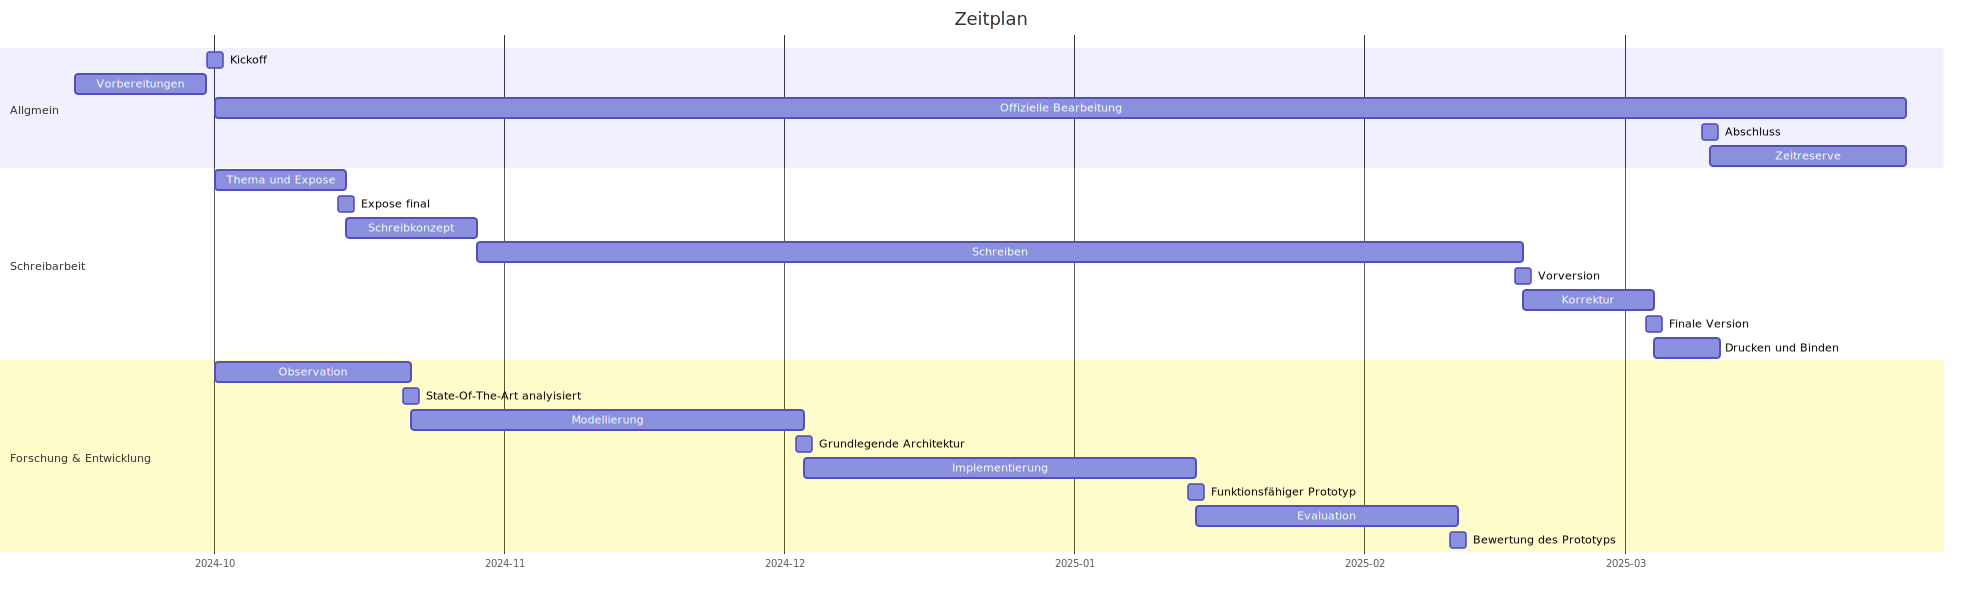
\includegraphics[width=1\textwidth]{Images/Gantt.png}
  \caption{Vorläufiger Zeitplan}
  \label{fig:gantt}
\end{figure}

\section{Ausgangsliteratur}
\printbibliography[title={""}]

\section{Abschlussarbeit im Unternehmen}

Die Abschlussarbeit soll bei der PACETEQ GmbH in Affalterbach durchgeführt werden.

Die Betreuung übernimmt Dominic Barth (M.Sc. Mechatronik).

\end{document}
